\newpage
\section{CASOS DE USO E DIAGRAMAS}
A criação dos diagramas junto com os casos de uso foram baseados nos arquivos artefatos disponibilizados para pesquisa no trabalho. Utilizamos nossos requisitos para aperfeiçoar os diagramas disponíveis de acordo com as necessidades que estipulamos. Os três casos de uso e seus diagramas estão disponíveis a seguir.

% ----------------------------------------------------------------------------------------------------------

\subsection{Diagrama geral de casos de uso}

Na figura \ref{fig:diagramaGeral} está o diagrama que aborda os casos de uso da plataforma a ser desenvolvida. É a partir dele que serão apresentados diagramas de casos de uso mais específicos abaixo.

\begin{figure}[h]
    \centering
    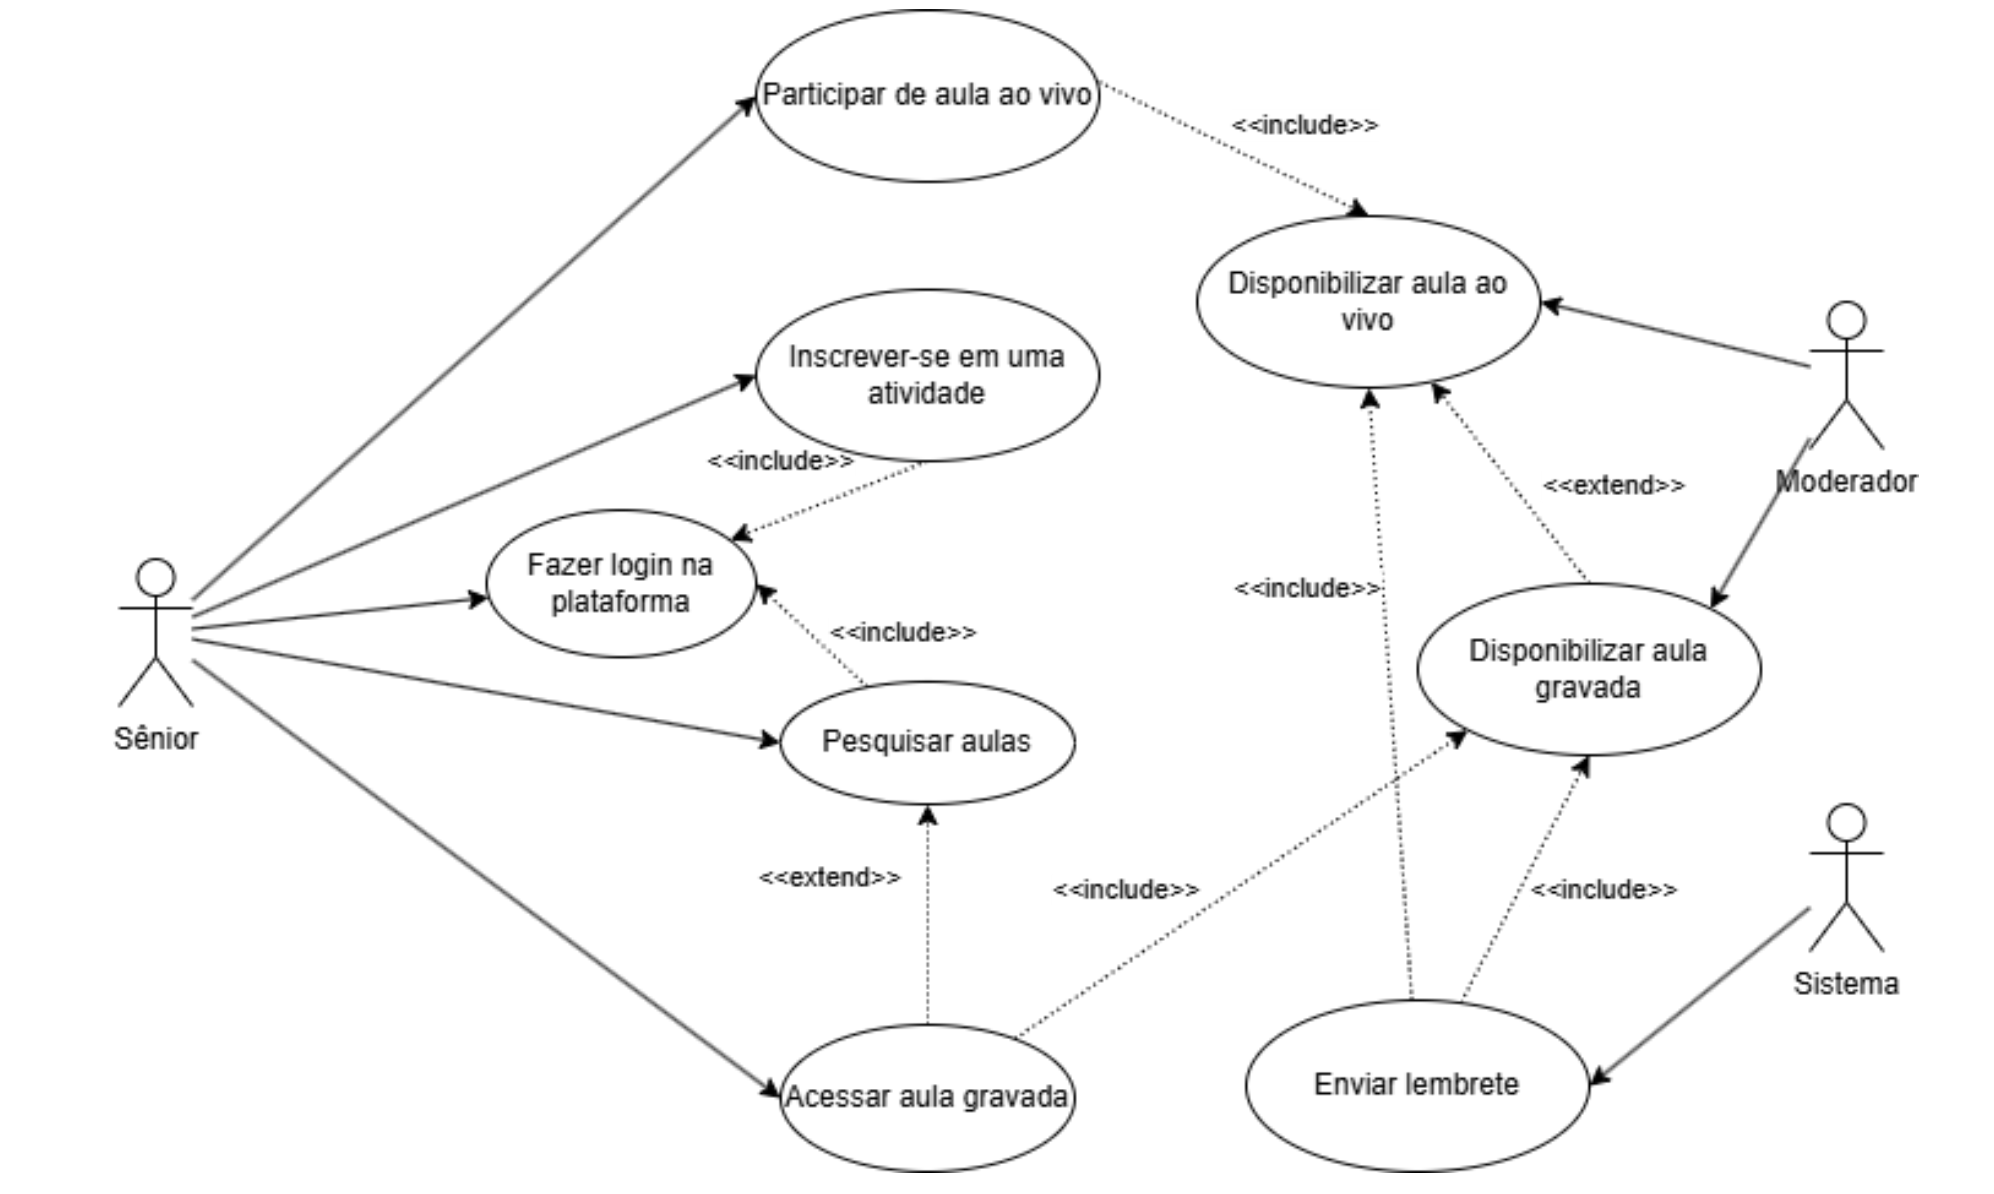
\includegraphics[width=0.8\linewidth]{images/diagramaGeral.png}
    \caption{Diagrama 1}
    \label{fig:diagramaGeral}
\end{figure}

\subsection{Assistir à aula gravada}

\begin{figure}[h]
    \centering
    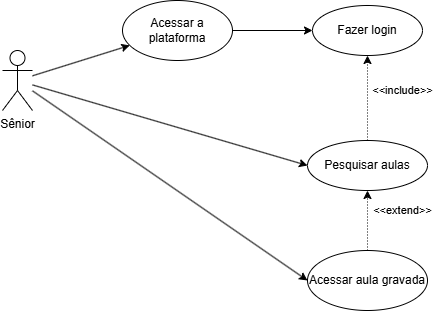
\includegraphics[width=0.8\linewidth]{images/diagrama1.png}
    \caption{Diagrama 1}
    \label{fig:diagrama1}
\end{figure}

\textbf{Atores:} Sênior

\vspace{\baselineskip}
\textbf{Descrição: } Permite ao sênior acessar a aula gravada em caso de ausência na aula síncrona.

\vspace{\baselineskip}
\textbf{Pré-condições: }
\begin{itemize}
    \item A aula gravada deve existir na plataforma.
    \item O sênior precisa estar cadastrado no sistema.
    \item O sistema que disponibiliza o vídeo deve estar funcionando.
\end{itemize}

\vspace{\baselineskip}
\textbf{Fluxo Principal: }
\begin{enumerate}
    \item O sênior acessa a plataforma;
    \item O sênior realiza o login;
    \item O sênior pesquisa as aulas disponíveis;
    \item O sênior seleciona e acessa a aula gravada desejada;
    \item O sistema carrega o vídeo e o reproduz;
\end{enumerate}

\vspace{\baselineskip}
\textbf{Fluxos Alternativos: }
\begin{itemize}
    \item 2.a - O sênior não possui cadastro na plataforma → O sistema redireciona para o cadastro.
\end{itemize}

\vspace{\baselineskip}
\textbf{Pós-condições: }
\begin{itemize}
    \item O sênior assiste à aula gravada;
    \item O vídeo fica sinalizado como assistido na plataforma;
\end{itemize}

% ----------------------------------------------------------------------------------------------------------

\subsection{Disponibilizar uma aula gravada}
\begin{figure}[H]
    \centering
    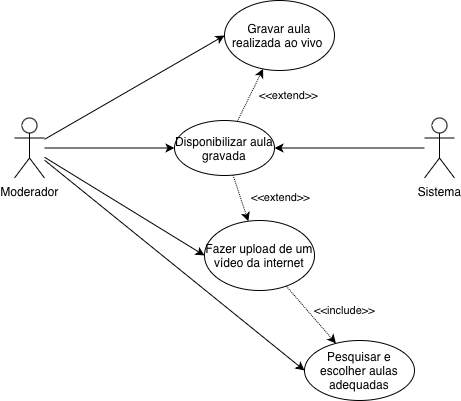
\includegraphics[width=0.8\linewidth]{images/diagrama2.png}
    \caption{Diagrama 2}
    \label{fig:diagrama2}
\end{figure}

\textbf{Atores:} Moderador, Sistema.

\vspace{\baselineskip}
\textbf{Descrição: } Permite ao moderador disponibilizar uma aula gravada para ser assistida por seniors na plataforma. Ele pode fazer isso gravando uma aula ao vivo ou pegando um vídeo da internet.

\vspace{\baselineskip}
\textbf{Pré-condições: }
\begin{itemize}
    \item Pode ou não ter acontecido uma aula ao vivo.
    \item O vídeo precisa ou não estar disponível na internet.
    \item O sistema deve estar funcionando.
\end{itemize}

\vspace{\baselineskip}
\textbf{Fluxo Principal: }
\begin{enumerate}
    \item O moderador grava a aula ao vivo que está realizando;
    \item O moderador faz upload do vídeo gravado na plataforma;
    \item O moderador disponibiliza esse vídeo para acesso dos seniors;
    \item O sistema deixa o vídeo exposto e disponível para os seniors.
\end{enumerate}

\vspace{\baselineskip}
\textbf{Fluxos Alternativos: }
\begin{itemize}
    \item 1.a - O moderador não realizou aula ao vivo - ele pode encontrar uma adequada na internet.
\end{itemize}

\vspace{\baselineskip}
\textbf{Pós-condições: }
\begin{itemize}
    \item Um novo vídeo é adicionado à plataforma.
    \item Os seniors são notificados da atualização.
\end{itemize}

% ----------------------------------------------------------------------------------------------------------

\subsection{Participar de encontro ao vivo}
\begin{figure}[H]
    \centering
    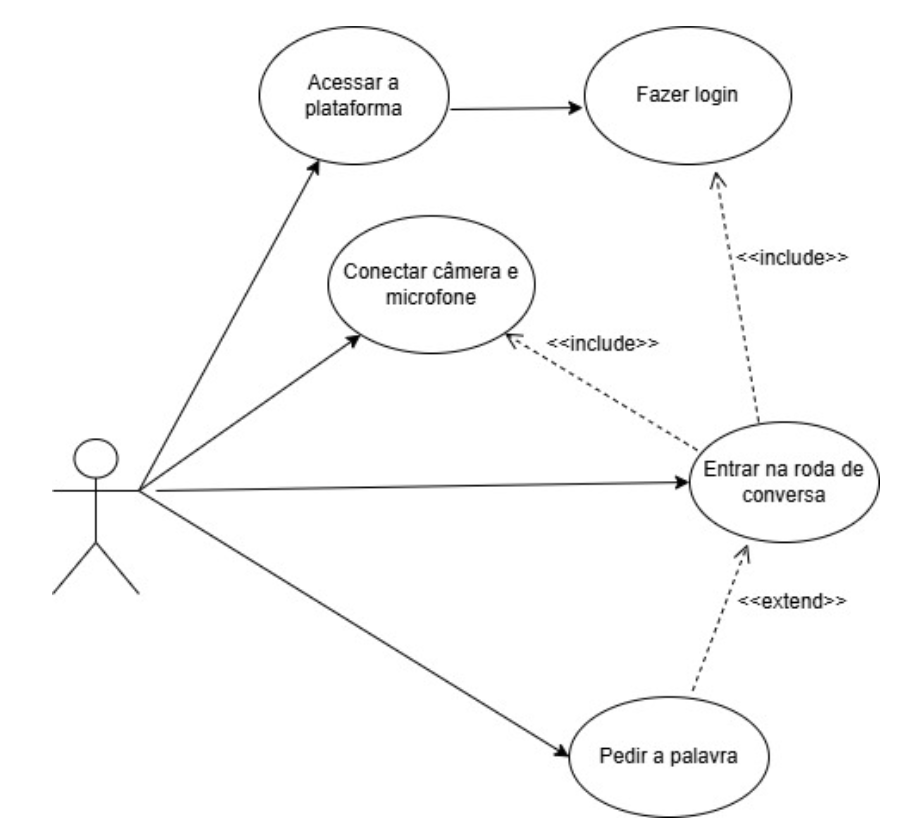
\includegraphics[width=0.8\linewidth]{images/diagrama3.png}
    \caption{Diagrama 3}
    \label{fig:diagrama3}
\end{figure}

\textbf{Atores:} Sênior

\vspace{\baselineskip}
\textbf{Descrição: } Permite ao sênior acessar e assistir a um encontro que está sendo transmitido em tempo real na plataforma. Ele pode ingressar na sala virtual, acompanhar o conteúdo e interagir durante a transmissão. 

\vspace{\baselineskip}
\textbf{Pré-condições: }
\begin{itemize}
    \item O sênior deve estar logado na plataforma.
    \item O sistema deve estar funcionando com a infraestrutura de transmissão de vídeo ativa. 
\end{itemize}

\vspace{\baselineskip}
\textbf{Fluxo Principal: }
\begin{enumerate}
    \item O sênior acessa a plataforma;
    \item O sênior realiza o login;
    \item O sênior entra no encontro ao vivo;
    \item O sistema conecta o dispositivo do sênior (áudio e vídeo) à sala de transmissão;
    \item O sistema exibe o vídeo e o áudio do encontro na tela do sênior;
    \item O sênior participa do encontro ao vivo.
\end{enumerate}

\vspace{\baselineskip}
\textbf{Fluxos Alternativos: }
\begin{itemize}
    \item 6.a - O sênior deseja interagir no encontro, pedindo a palavra,  e o sistema repassa a interação.
\end{itemize}

\vspace{\baselineskip}
\textbf{Pós-condições: }
\begin{itemize}
    \item O sênior participou e visualizou o conteúdo do encontro ao vivo. 
    \item O sistema registra a presença e o histórico de participação do sênior na plataforma.
\end{itemize}